\section{Introduction}

There has been growing research on LLM inference optimization. In particular, recent
work~\cite{liu2025optimizingllmqueriesrelational, cheng2025letbarbariansinai}
presents solutions to optimize relational data analytics workloads for offline LLM inference.
It proposes Greedy Group Recursion (GGR), an approximate algorithm that leverages
functional dependencies (such as primary and foreign key relationships from the data
schema) and table statistics, which are readily available in many databases and
analytics systems, to reduce the search space.

% @formatter:off
\begin{algorithm}[t!]
\caption{Greedy Group Recursion (GGR)}
\begin{algorithmic}[1]
\small
\STATE \textbf{Input:} Table $T$, Functional Dependency $FD$
\STATE \textbf{Output:} Prefix Hit Count $S$, Reordered List of Tuples $L$


\item[]
\FUNCTION{$\textsc{HitCount} (v, c, T, FD)$}
    \STATE $R_v \gets \{i \mid T[i,c] = v\}$
    \STATE $\text{inferred\_cols} \gets \{c' \mid (c, c') \in FD\}$
    \STATE $\text{inferred\_vals} \gets \{T[R_v[1], c'] \mid c' \in \text{inferred\_cols}\}$
    \STATE $\text{tot\_len} \gets \text{len}(v)^2 + \sum_{\substack{c' \in \text{inferred\_cols}}} \left( \frac{\sum_{r \in R_v} \text{len}(T[r, c'])}{|R_v|} \right)^2$
    \STATE $HC \gets \text{tot\_len} \times (|R_v| - 1)$
    \STATE $cols \gets [c] + \text{inferred\_cols}$
    \STATE $vals \gets [v] + \text{inferred\_vals}$
    \STATE \textbf{return} $HC, cols, vals$
\ENDFUNCTION


\item[]
\FUNCTION{\textsc{GGR}($T$, $FD$)}
    % \IF{$|T|_{rows} = 1$ or $|T|_{cols} = 1$}
    %     \STATE \textbf{return } \text{Base case processing as in \optimal}
    % \ENDIF
    \IF{$|T|_{rows} = 1$}
        \STATE {\bfseries return} $0, [T[1]]$
    \ENDIF
    \IF{$|T|_{cols} = 1$}
        \STATE $S \gets \sum_{v \in \text{distinct}(T[,1])} \textsc{HitCount}(v, 1, T)$ % groupby or sort, choose best group, append
        \STATE {\bfseries return} $S, sort([T[i] \mid i \in 1 \dots |T|_{rows}])$
    \ENDIF

    \STATE $b\_v, b\_c \gets \text{None}, \text{None}$
    \STATE $max\_HC, b\_cols, b\_vals \gets -1, [], []$

    \FOR{$c \in \text{columns}(T)$, $v \in \text{distinct}(T[,c])$}
        \STATE $HC, cols, vals \gets \textsc{HitCount}(v, c, T, FD)$
        \IF{$HC > max\_HC$}
            \STATE $b\_v, b\_c \gets v, c$
            \STATE $max\_HC, b\_cols, b\_vals \gets HC, cols, vals$
        \ENDIF
    \ENDFOR

    \STATE $R\_v \gets \{i \mid T[i, b\_c] = b\_v\}$
    \STATE $A\_HC, A\_L \gets \textsc{GGR}(T[\text{rows} \setminus R\_v, \text{cols}], FD)$
    \STATE $B\_HC, B\_L \gets \textsc{GGR}(T[R\_v, \text{cols} \setminus b\_cols], FD)$
    \STATE $C\_HC \gets max\_HC$
    \STATE $S \gets A\_HC + B\_HC + C\_HC$
    \STATE $L \gets [b\_vals + B\_L[i] \mid i \in 1 \dots |R\_v|] + A\_L$
    \STATE \textbf{return} $S, L$
\ENDFUNCTION

\item[]
\STATE \textbf{return} \textsc{GGR}($T$, $FD$)
\end{algorithmic}
\label{alg:greedy}
\end{algorithm}
% @formatter:on


\vspace{-0.5em}

\subsection{Greedy Group Recursion (GGR) Algorithm} \label{sec:ggr}

The GGR algorithm is described in detail in~\cite{liu2025optimizingllmqueriesrelational}.
Let us briefly outline its main points.

The pseudocode specification of GGR is in Algorithm~\ref{alg:greedy} listing and is
taken from the original paper but with several critical corrections
(and multiple little typo fixes).

GGR algorithm optimizes LLM queries by finding a ($n \times m$) table rearrangement
that maximizes the LLM's KV cache prefix hit count (PHC).
It achieves this goal by reordering the rows and the fields within each row.
Each row may have a different field order.
The rearranged table is represented as a list of tuples $L$, where each tuple
in $L$ corresponds to a row, and the tuple elements contain the column values.
A cell in the list of tuples is denoted as $L[r][f]$, indicating the value in tuple $r$ at position $f$.

\vspace{-0.5em}

\subsubsection{Prefix Hit Count Calculation}

The hit count of a single cell $L[r][c]$ is non-zero \textbf{only} if its value is
the same as in the previous row $L[r][c] = L[r-1][c]$ \textbf{and} all preceding
fields have the same property $\forall f \leq c, L[r][f] = L[r-1][f]$.
Then its hit count is computed as the square of the value's string length:

\vspace{-1.5em}
\begin{equation}
    \textit{hit}(L, r, c) =
    \begin{cases}
        \text{len}(L[r][c])^2 & \text{if } \forall f \leq c, \\ & L[r][f]= \\ & L[r-1][f] \\
        0 & \text{otherwise}
    \end{cases}
    \label{eq:cellhit}
\end{equation}
\vspace{-1.5em}

The squared string length reflects the quadratic complexity of token processing in
LLM inference, where each token computation depends on every preceding token and
increases computational cost quadratically with the input length.

The hit count for a single row $r$ in $L$ is then just a sum of hit counts for all
cells in a row:

\vspace{-1.5em}
\begin{equation}
    \textit{hit}(L, r) = \sum_{c=1}^{m} \textit{hit}(L, r, c)
    \label{eq:rowhit}
\end{equation}
\vspace{-1.5em}

The PHC for a list of tuples $L$ with $n$ rows and $m$ fields is given by:

\vspace{-1.5em}
\begin{equation}
    \text{PHC}(L) = \sum_{r=1}^{n} \textit{hit}(L, r)
    \label{eq:phc}
\end{equation}
\vspace{-1.5em}

The $\text{PHC}(L)$ is the objective function of a table reordering algorithm: it
tries to find output $L$ with maximum $\text{PHC}(L)$ value.

\vspace{-0.5em}

\subsubsection{Selecting the highest-hit distinct value}

The greedy part of GGR is based on finding a distinct value $v$
(in the corresponding column $c$) with the highest hit count among all distinct
values in the table $T$.
If $R_v = R(v, c, T)$ are the rows with value $v$ in the column $c$:

\vspace{-1.5em}
\begin{equation}
    R(v, c, T) = \{i \mid T[i,c] = v\},
    \label{eq:vcrows}
\end{equation}
\vspace{-1.5em}

then hit count of $v, c$ is given by:

\vspace{-1.5em}
\begin{equation}
    \textit{HitCount}(v, c, T) = \text{len}(v)^2 \times (|R(v, c, T)| - 1)
    \label{eq:hitcount}
\end{equation}
\vspace{-1.5em}

GGR then places all $v, c$ cells in consecutive rows and in the first field of the
output $L$ and splits remaining cells of the table $T$ into the sub-table of
rows $R_v$ with excluded column $c$: $T[R_v, \text{cols} \setminus [c]]$,
and the sub-table of rows excluding $R_v$: $T[\text{rows} \setminus R_v, \text{cols}]$.
GGR then recursively runs on each of two sub-tables.
See Figure~\ref{fig:optimal} for illustration of this key step.

Compared to the brute-force algorithm that
requires $n! \times (m!)^n$ potential orderings, GGR significantly reduces the search
space by selecting the highest-hit value and then reducing the dimensions of the
table at each recursive step with the maximum depth of recursion $O(\min(n,m))$.
GGR achieves close-to-perfect PHC output with fast practical execution time.

\vspace{-0.5em}

\subsubsection{Functional Dependencies}

GGR algorithm leverages a table's functional dependencies (FD) to reduce the number
of fields it needs to consider at each recursion step.

We say that two columns $A$ and $B$ are in functional dependency $A \leftrightarrow B$
in a table $T$ if, for any two rows $r_1$ and $r_2$, $T[r_1, A] = T[r_2, A]$ implies
$T[r_1, B] = T[r_2, B]$ and vice versa.

In other words, for any distinct value $a$ in the column $A$, there is a distinct
value $b$ in the column $B$ such that they both are on the same rows.
I.e., for $R_a \gets \{i \mid T[i,A] = a\}$ and $R_b \gets \{i \mid T[i,B] = b\}$ we have
$R_a = R_b$.

FD rules can be specified as a list of disjoint sets containing column indices.
For example, for the table with columns $A, B, C, D, E, F$ where
$A \leftrightarrow B$ and $C \leftrightarrow D \leftrightarrow E$, the FD rules can
be written as $[[A, B], [C, D, E]]$.

GGR takes advantage of FD by combining distinct values from columns in the same FD
rule into one block of value groups.
See Figure~\ref{fig:optimal-fd} for illustration of GGR iteration in the presence of FD rule.

\begin{figure}
    \centering
%    \includegraphics[width=0.49\textwidth]{figures/MLSys_Figures/prefix_hit_maximization}
    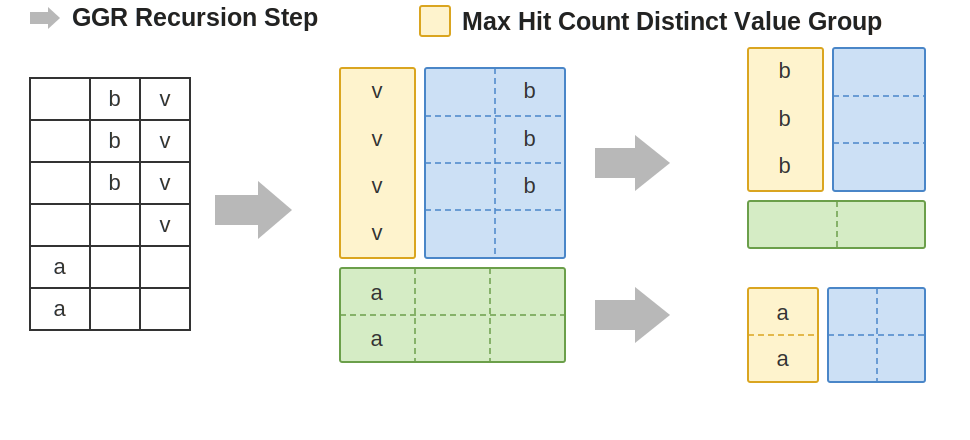
\includegraphics[width=0.49\textwidth]{figures/claude-figures/max_hit_recursion}
    \vspace{-1.5em}
    \caption{
        GGR picks the group with the maximum hit count at each step and calculates PHC
        as the sum of PHC of the elected group values (yellow box),
        the sub-table $T$ excluding rows $R_v$ (green box),
        and the sub-table of rows $R_v$ excluding the field where the value is located in (blue box).
        In the input table $T$ (white box on the left), $HitCount(v) > HitCount(b) > HitCount(a)$
        and all other distinct values have hit count zero.
    }
    \label{fig:optimal}
    \vspace{-1.5em}
\end{figure}

\vspace{-0.5em}

\subsubsection{GGR Specification}

We can follow the pseudocode specification of GGR in Algorithm~\ref{alg:greedy} listing.

At each recursive step, the GGR algorithm scans the table (lines 21--29) to find
all distinct values with corresponding hit counts (lines 3--12).
It then selects the highest-hit value $b\_v$ (in the column $b\_c$) and splits the
table into two sub-tables - one with all the rows $R\_v$ containing $b\_v$ value
but excluding the column $b\_c$ and its FD-associated columns
(line 31: $T[R\_v, \text{cols} \setminus b\_cols]$),
and another sub-table with the remaining rows
(line 32: $T[\text{rows} \setminus R\_v, \text{cols}]$).
In the final step, GGR recurses on the two sub-tables (lines 31--32) and calculates
the total PHC as the sum of PHCs computed for each sub-table and of hit count
computed for $b\_v, b\_c$ (line 34).

There are two recursion termination conditions:
\vspace{-0.5em}
\begin{itemize}
    \item When a table contains only a single row. Then PHC is zero and the table is
    not rearranged. (Lines 14--16.)
    \item When a table contains only a single column. Then the table with sorted
    column values is returned and PHC is trivially computed. (Lines 17--20.)
\end{itemize}

\begin{figure}
    \centering
    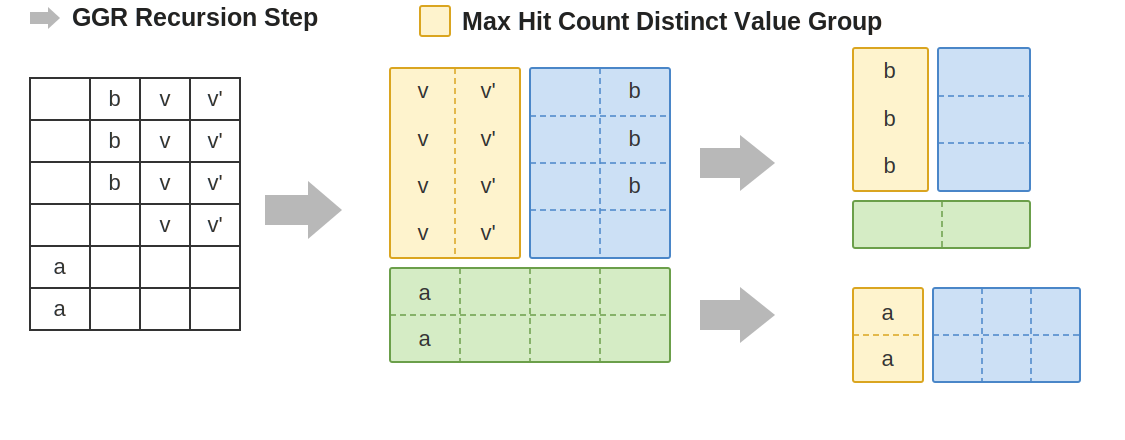
\includegraphics[width=0.49\textwidth]{figures/claude-figures/max_hit_recursion_vprime}
    \vspace{-1.5em}
    \caption{
        Similar to Figure~\ref{fig:optimal} but with two distinct values $v$ (in column $c$)
        and $v'$ (in column $c'$) bound by FD rule $FD = [c, c']$.
        In the input table $T$ (white box on the left),
        $HitCount(v) + HitCount(v') > HitCount(b) > HitCount(a)$
        and all other distinct values have hit count zero.
    }
    \label{fig:optimal-fd}
    \vspace{-1.5em}
\end{figure}

\vspace{-0.5em}

\subsubsection{Optimality of GGR Algorithm}

While GGR approximates the ideal optimal rearrangement of rows and columns, it can
achieve \textit{proven} optimal PHC in certain cases.

The first case is a trivial one -- when hit counts of all distinct values
(with FD accounted for) are zero.
It means that every distinct value in the table appears in a single row only.
In this case non-zero PHC cannot be achieved by any table rearrangement.
This case also covers one of the recursion termination conditions -- a table with a single row.

The second case is when all columns of a table are bound by an FD rule.
In other words, any column functionally determines all other columns.
In this case for each distinct value GGR combines all columns to one group of values,
capturing all key correlations and producing the optimal reordering.
This case also covers the recursion termination conditions -- a table with a single column.

However, there are cases when GGR clearly produces suboptimal solutions.

One case is when distinct values tie in max hit count.
See an example of this case with GGR producing suboptimal reordering in Figure~\ref{fig:suboptimal-ex-1}.

\begin{figure}
    \centering
    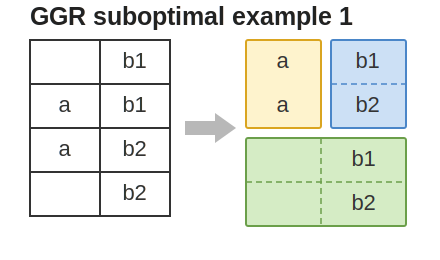
\includegraphics[width=0.49\textwidth]{figures/claude-figures/subopt-example-1-ties}
    \vspace{-1.5em}
    \caption{
        Example of a table with max hit count ties and suboptimal GGR output.
        $HitCount(a) = HitCount(b1) = HitCount(b2)$
    }
    \label{fig:suboptimal-ex-1}
%    \vspace{-1.5em}
\end{figure}

Another case is when a distinct value in one column correlates with a distinct value
in another column.
This is not the case of FD-bound columns (even though it might sound similar),
but, rather, the case of data heuristics when two distinct values in two columns
happen to share the same rows.
See an example of this case with GGR producing suboptimal reordering in Figure~\ref{fig:suboptimal-ex-2}.

\begin{figure}
    \centering
    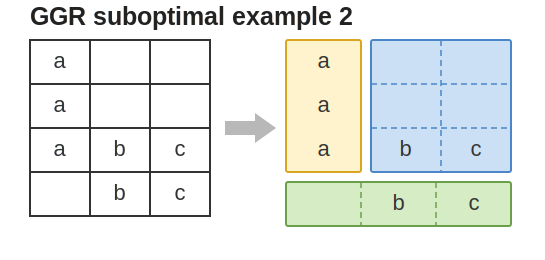
\includegraphics[width=0.49\textwidth]{figures/claude-figures/subopt-example-2-corrs}
    \vspace{-1.5em}
    \caption{
        Example of a table with correlated distinct values $b$ and $c$, and suboptimal GGR output.
        $HitCount(a) = HitCount(b) + HitCount(c)$ and $R_b = R_c$
    }
    \label{fig:suboptimal-ex-2}
    \vspace{-1.5em}
\end{figure}

\vspace{-0.5em}

\subsection{Reference Implementation of GGR Algorithm} \label{sec:ggr-impl}

The reference implementation of GGR specification from Algorithm~\ref{alg:greedy}
can be found in~\cite{ggrimpl}.
